\documentclass[a4paper, 12pt]{article}

\usepackage[margin=1in]{geometry}
\usepackage{amsmath, amsfonts, amssymb}
\usepackage{booktabs}
\usepackage{graphicx}
\usepackage{hyperref}
\usepackage{titlesec}
\usepackage{tabularx}
\usepackage{makecell}
\usepackage{array}
\usepackage{multirow}
\usepackage{listings}
\usepackage{enumitem}

\title{\Large\textbf{Optimization Algorithms: Steepest Descent vs. Conjugate Gradient}}
\author{Rushil Gupta}
\date{}

\lstset{
    basicstyle=\ttfamily\small,
    breaklines=true,
    frame=single,
    numbers=left,
    numbersep=5pt
}

\begin{document}

\maketitle

\section*{Introduction}

This document presents an analysis of two optimization algorithms—Steepest Descent and Conjugate Gradient—applied to the quadratic function:

\[
f(\mathbf{x}) = \frac{1}{2} \mathbf{x}^T A \mathbf{x} - \mathbf{b}^T \mathbf{x},
\]

where \( A \) is a symmetric positive-definite matrix, \( \mathbf{b} \) is a constant vector, and \( \mathbf{x} \) is the variable vector. The goal is to find the vector \( \mathbf{x}^* \) that minimizes \( f(\mathbf{x}) \).

\section*{Methodology}

Both algorithms aim to iteratively approach the optimal solution \( \mathbf{x}^* \) by minimizing the function \( f(\mathbf{x}) \). Below are the detailed steps for each method:

\subsection*{Steepest Descent}

The Steepest Descent method updates the solution by moving in the direction of the negative gradient of the function. The algorithm proceeds as follows:

\begin{enumerate}
    \item \textbf{Initialization}: Start with an initial guess \( \mathbf{x}_0 \).
    \item \textbf{Compute Gradient}: Calculate the gradient \( \mathbf{r} = \nabla f(\mathbf{x}) = A\mathbf{x} - \mathbf{b} \).
    \item \textbf{Check Convergence}: If \( \|\mathbf{r}\| < \text{tol} \), terminate the algorithm.
    \item \textbf{Determine Step Size}: Compute the optimal step size \( \alpha = \frac{\mathbf{r}^T \mathbf{r}}{\mathbf{r}^T A \mathbf{r}} \).
    \item \textbf{Update Solution}: Update the solution \( \mathbf{x} = \mathbf{x} - \alpha \mathbf{r} \).
    \item \textbf{Repeat}: Return to step 2 until convergence or the maximum number of iterations is reached.
\end{enumerate}

\subsection*{Conjugate Gradient}

The Conjugate Gradient method enhances the Steepest Descent by ensuring that each search direction is conjugate to the previous ones, leading to faster convergence for quadratic functions. The algorithm is as follows:

\begin{enumerate}
    \item \textbf{Initialization}: Start with an initial guess \( \mathbf{x}_0 \), compute the initial residual \( \mathbf{r}_0 = \mathbf{b} - A\mathbf{x}_0 \), and set the initial search direction \( \mathbf{p}_0 = \mathbf{r}_0 \).
    \item \textbf{Iteration}: For each iteration \( k \):
    \begin{enumerate}[label=\roman*)]
        \item \textbf{Compute Step Size}: \( \alpha_k = \frac{\mathbf{r}_k^T \mathbf{r}_k}{\mathbf{p}_k^T A \mathbf{p}_k} \).
        \item \textbf{Update Solution}: \( \mathbf{x}_{k+1} = \mathbf{x}_k + \alpha_k \mathbf{p}_k \).
        \item \textbf{Update Residual}: \( \mathbf{r}_{k+1} = \mathbf{r}_k - \alpha_k A \mathbf{p}_k \).
        \item \textbf{Check Convergence}: If \( \|\mathbf{r}_{k+1}\| < \text{tol} \), terminate the algorithm.
        \item \textbf{Compute Beta}: \( \beta_k = \frac{\mathbf{r}_{k+1}^T \mathbf{r}_{k+1}}{\mathbf{r}_k^T \mathbf{r}_k} \).
        \item \textbf{Update Search Direction}: \( \mathbf{p}_{k+1} = \mathbf{r}_{k+1} + \beta_k \mathbf{p}_k \).
    \end{enumerate}
    \item \textbf{Repeat}: Continue until convergence or the maximum number of iterations is reached.
\end{enumerate}

\section*{Results}

Both algorithms were executed on the following system:

\begin{itemize}
    \item \textbf{Matrix \( A \)}:
    \[
    A = \begin{bmatrix}
    4 & 1 \\
    1 & 3 \\
    \end{bmatrix}
    \]
    \item \textbf{Vector \( \mathbf{b} \)}:
    \[
    \mathbf{b} = \begin{bmatrix}
    1 \\
    2 \\
    \end{bmatrix}
    \]
    \item \textbf{Initial Guess \( \mathbf{x}_0 \)}:
    \[
    \mathbf{x}_0 = \begin{bmatrix}
    2 \\
    1 \\
    \end{bmatrix}
    \]
    \item \textbf{Tolerance}: \( \text{tol} = 1 \times 10^{-8} \)
    \item \textbf{Maximum Iterations}: 1000
\end{itemize}

\subsection*{Optimal Solutions and Performance}

\begin{table}[h]
    \centering
    \caption{Optimization Results}
    \begin{tabular}{@{}llll@{}}
        \toprule
        \textbf{Method} & \textbf{Optimal \( \mathbf{x} \)} & \textbf{\( f(\mathbf{x}^*) \)} & \textbf{Iterations} \\ \midrule
        Steepest Descent & $[0.0909, 0.6364]$ & $-0.6818$ & 11 \\
        Conjugate Gradient & $[0.0909, 0.6364]$ & $-0.6818$ & 2 \\
        \bottomrule
    \end{tabular}
\end{table}

\newpage
\subsection*{Convergence Plot}

The convergence behavior of both algorithms is illustrated in Figure~\ref{fig:convergence}.

\begin{figure}[h]
    \centering
    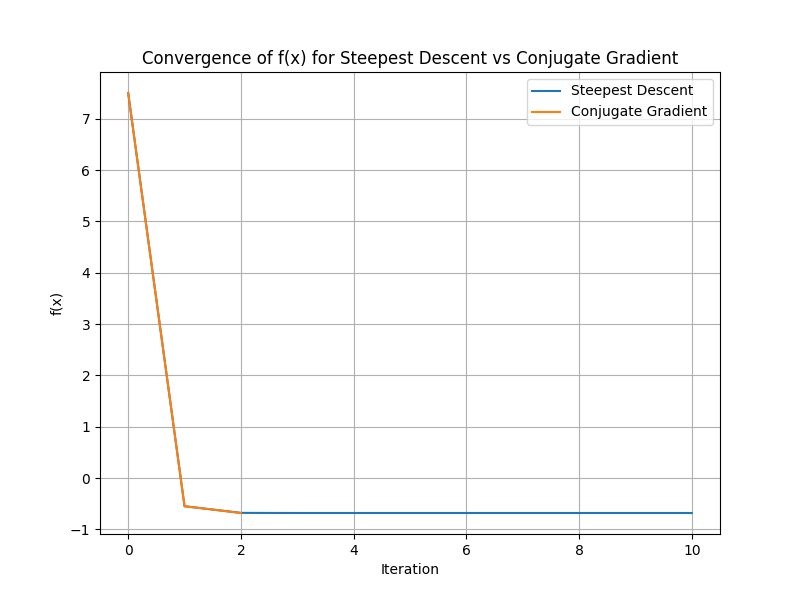
\includegraphics[width=0.8\textwidth]{Convergence.png}
    \caption{Convergence of \( f(\mathbf{x}) \) for Steepest Descent vs. Conjugate Gradient}
    \label{fig:convergence}
\end{figure}

\section*{Discussion}

The results indicate that:

\begin{itemize}
    \item \textbf{Optimal Solutions}: Both algorithms successfully converged to the optimal solution \( \mathbf{x}^* \), achieving similar function values \( f(\mathbf{x}^*) \).
    \item \textbf{Iterations}: The Conjugate Gradient method required significantly fewer iterations to converge compared to the Steepest Descent method.
\end{itemize}

\section*{Conclusion}

Both Steepest Descent and Conjugate Gradient methods are effective for minimizing quadratic functions. However, the Conjugate Gradient method outperforms Steepest Descent in terms of the number of iterations required to reach convergence.

\end{document}